% ================================================================
% MITS-006 - Mobile Programming
% Course Project Research Paper
% University of the Immaculate Conception, Philippines
% College of Computer Studies
%
% PEAM-Registry: Provincial Event Attendance and Mobile Registry
%
% Files expected in the same folder:
%   main.tex
%   references.bib
%   concept.png
%   userjourney.png
%   wireframe.png
%
% Compile with Biber: LaTeX -> Biber -> LaTeX -> LaTeX.
%
% Usability results that are still being collected are marked with
% \pending{...}. Replace each one after the evaluation sessions.
% ================================================================

\documentclass[conference]{IEEEtran}

% ---------- Bibliography ----------
\usepackage[
    backend=biber,
    style=ieee,
    sorting=none
]{biblatex}
\addbibresource{references.bib}

% ---------- General packages ----------
\usepackage{graphicx}
\usepackage{amsmath,amssymb}
\usepackage{booktabs}
\usepackage{array}
\usepackage{tabularx}
\usepackage{algorithm}
\usepackage{algpseudocode}
\usepackage{url}
\usepackage[hidelinks]{hyperref}

% ---------- Safer table column types ----------
\newcolumntype{Y}{>{\raggedright\arraybackslash}X}
\newcolumntype{P}[1]{>{\raggedright\arraybackslash}p{#1}}

% ---------- Student Guide Questions ----------
\newif\ifstudentguide
\studentguidefalse

\newcommand{\guide}[1]{%
    \ifstudentguide
        \par\smallskip
        \noindent
        \begin{minipage}{\columnwidth}
        \small\itshape
        \textbf{Guide questions:} #1
        \end{minipage}
        \par\smallskip
    \fi
}

% Values that will be filled in after the usability sessions.
\newcommand{\pending}[1]{\textbf{[#1]}}

\begin{document}

% ================================================================
% TITLE AND AUTHORS
% ================================================================

\title{PEAM-Registry: A Mobile Attendance System Using GPS Event Areas,
On-Device Biometrics, and Offline Synchronization for Provincial
Government Events in Davao del Sur}

\author{
\IEEEauthorblockN{Clyde Chester Balaman}
\IEEEauthorblockA{
\textit{College of Computer Studies}\\
\textit{University of the Immaculate Conception}\\
Davao City, Philippines\\
cbalaman@uic.edu.ph
}
\and
\IEEEauthorblockN{Harold Beltran}
\IEEEauthorblockA{
\textit{College of Computer Studies}\\
\textit{University of the Immaculate Conception}\\
Davao City, Philippines\\
hbeltran@uic.edu.ph
}
}

\maketitle

% ================================================================
% ABSTRACT
% ================================================================

\begin{abstract}
Employees of the Provincial Government of Davao del Sur attend
assemblies, trainings, and outreach activities inside and outside the
Capitol. Recording attendance at these events depends on physical
biometric scanners that must be transported, powered, and configured at
each venue, or on paper logbooks that cannot prove who signed or where.
This project developed the Provincial Event Attendance and Mobile
Registry (PEAM-Registry), a Flutter mobile application backed by
Supabase and paired with a web console for the human resource office.
An employee signs in with an Employee ID and a one-time code sent to the
work email on file, and the first phone used is registered as the only
phone allowed for attendance. To check in, the application confirms that
the event has started, measures the distance between the phone and the
venue, and allows the attendance only inside the event area set by human
resources. The phone's own fingerprint or face unlock then confirms the
user; no fingerprint or face data leaves the phone. Records are saved on
the phone first and sent to the server automatically when the connection
returns, and employees receive reminders, including a reminder to check
out while the event is still running. The system was built through
iterative development and verified with 78 automated unit and widget
tests, all of which passed. A task-based usability evaluation using the
System Usability Scale has been designed for provincial employees. The
project shows that ordinary smartphones can replace transported scanners
for off-site government events while keeping attendance tied to a
person, a place, and a time.
\end{abstract}

\begin{IEEEkeywords}
mobile attendance, geofencing, biometric authentication, offline-first,
Flutter, Supabase, e-government
\end{IEEEkeywords}

% ================================================================
% I. INTRODUCTION
% ================================================================

\section{Introduction}

\subsection{Background and Context}

The Provincial Government of Davao del Sur regularly gathers its
employees for official events: the annual employees' assembly, flag
ceremonies, trainings, disaster drills, and outreach programs in the
municipalities. Attendance at these events is part of an employee's
official record and is reviewed by the provincial human resource office
(PHRMO).

At the Capitol, attendance is captured by wall-mounted biometric
scanners. For events held elsewhere, staff must carry a scanner to the
venue, find power, configure it for the event, and later download and
reconcile its logs. When a scanner is not available, attendance falls
back to paper sign-in sheets. Paper does not show that the person who
signed is the employee named, and it does not show that the employee was
actually at the venue. Both methods also delay the moment HR can see who
attended.

Most employees already carry a smartphone that contains the components
needed to verify attendance: a satellite positioning receiver, a secure
biometric sensor, local storage, and a network connection. Smartphone
positioning is accurate enough to distinguish being at a venue from
being elsewhere, although its error varies with the environment
\cite{zandbergen2009accuracy}. Modern mobile operating systems also
expose biometric confirmation through a system dialog, so an application
can confirm the device owner without handling any biometric data itself
\cite{androidbiometric}. Many provincial venues, however, have weak or
no mobile data, so any phone-based approach must keep working offline.

\subsection{Problem Statement}

The province lacks an attendance method for off-site events that is
portable, confirms both identity and presence, works without a reliable
connection, and gives HR timely records. Transported scanners are
costly in effort and equipment, and paper sheets are easy to falsify.
Employees are affected by long queues and lost records, and PHRMO is
affected by manual reconciliation and weak evidence. This project
addresses the question of how an employee's own phone can record
trustworthy attendance at a provincial event under these conditions.

\subsection{Research Objectives}

The general objective of this study is to develop and evaluate a mobile
attendance system that lets provincial employees record verified
attendance at official events using their own registered smartphones.

Specifically, the study aims to:
\begin{enumerate}
    \item design an attendance workflow that accepts a check-in only
    during the event and only inside the event area, confirms the user
    with the phone's built-in biometrics, and limits each employee to
    one registered phone;
    \item implement offline-first recording in which attendance is saved
    on the phone and synchronized automatically, producing exactly one
    record per employee per event;
    \item support HR through a shared backend, a web console, and push
    notifications for new events, event reminders, pending check-outs,
    and device-change decisions; and
    \item verify the system through automated functional tests and
    evaluate its usability with provincial employees using ISO 9241-11
    measures and the System Usability Scale.
\end{enumerate}

\subsection{Related Literature and Research Gap}

\textit{Location as proof of presence.}
Comparing a phone's reported position with a known venue coordinate is
a direct way to confirm presence. The great-circle distance between two
coordinates is computed reliably with the haversine formula
\cite{sinnott1984haversine}. The limit of the approach is the accuracy of
the position itself. Zandbergen found that assisted GPS on smartphones
is far more accurate than Wi-Fi or cell-tower positioning, but that
errors grow indoors and near tall structures
\cite{zandbergen2009accuracy}. A venue radius therefore has to be set
with some tolerance rather than at the size of the building.

\textit{Identity through device biometrics.}
Biometric recognition links an action to a person rather than to a
password or card \cite{jain2004biometric}. Collecting fingerprint or face
templates centrally, as standalone scanners do, raises storage and
privacy obligations. NIST guidance treats a registered device unlocked by
a local biometric as a combination of something the user has and
something the user is, with the biometric match kept on the device
\cite{nist80063b}. Android's biometric dialog follows this model: the
application only learns whether the match succeeded
\cite{androidbiometric}. Security baselines for mobile applications
likewise recommend relying on platform authentication and keeping
secrets out of the client \cite{owaspmasvs}.

\textit{Offline-first data.}
Kleppmann et al.\ argue that applications should treat the copy on the
device as primary and synchronize with the server in the background, so
that work continues without a connection \cite{kleppmann2019localfirst}.
For attendance this matters because a record that fails to send must not
be lost or duplicated when it is sent again.

\textit{Usability of workplace tools.}
ISO 9241-11 defines usability as effectiveness, efficiency, and
satisfaction in a specified context of use \cite{iso9241_11}. The System
Usability Scale (SUS) gives a reliable satisfaction score from ten items
\cite{brooke1996sus}, and Bangor et al.\ provide benchmarks for
interpreting it \cite{bangor2008sus}. Studies of sample size show that
five to eight participants reveal most usability problems in a
formative test \cite{virzi1992subjects,nielsen1993model}.

\textit{Gap.}
These sources address location checking, device biometrics, offline
storage, and usability separately. In the provincial setting studied,
off-site attendance still relies on transported scanners or paper, and
no tool in use combines event-time and event-area checks, on-device
biometric confirmation, one registered phone per employee, offline
recording, and HR review in a single workflow. PEAM-Registry is designed
to fill that gap for this specific context.

\subsection{Scope and Delimitations}

The study covers employees of the Provincial Government of Davao del Sur
who attend official events, and PHRMO staff who manage those events. The
employee application is built with Flutter and targets Android first;
the same code builds for iOS, but push notifications are configured for
Android only. The employee application supports sign-in, phone
registration, the event list with search and filters, check-in and
check-out with location and biometric confirmation, offline storage and
synchronization, attendance history, notifications, and device-change
requests. HR functions such as creating events, setting the venue and
radius, reviewing attendance, and approving phone changes are handled in
a separate web console that shares the same backend.

The system does not compute pay, leave, or tardiness, and it does not
replace the Capitol's fixed scanners for daily time records. It does not
collect or store fingerprints or face images. It does not yet detect
spoofed or simulated locations, and it does not include liveness
detection or automated fraud analytics; these appear in the user journey
as future integrations.

% ================================================================
% II. METHODS
% ================================================================

\section{Methods}

\subsection{Research or Development Design}

The study uses a developmental design with an evaluative component. The
system was built iteratively in short cycles; each cycle added a feature
along the employee journey, wrote automated tests for its rules, and
revised the interface wording based on review. This approach suits the
objectives because the requirements, especially around offline
behavior and plain-language messages for employees of all ages, became
clearer as working versions were tried. The project proceeded through
five phases: requirements and process definition, data and interface
design, implementation, functional verification, and usability
evaluation.

\subsection{Conceptual Framework}

Figure~\ref{fig:conceptual_framework} presents the conceptual framework
of the study as an input--process--output model.

\begin{figure}[!t]
    \centering
    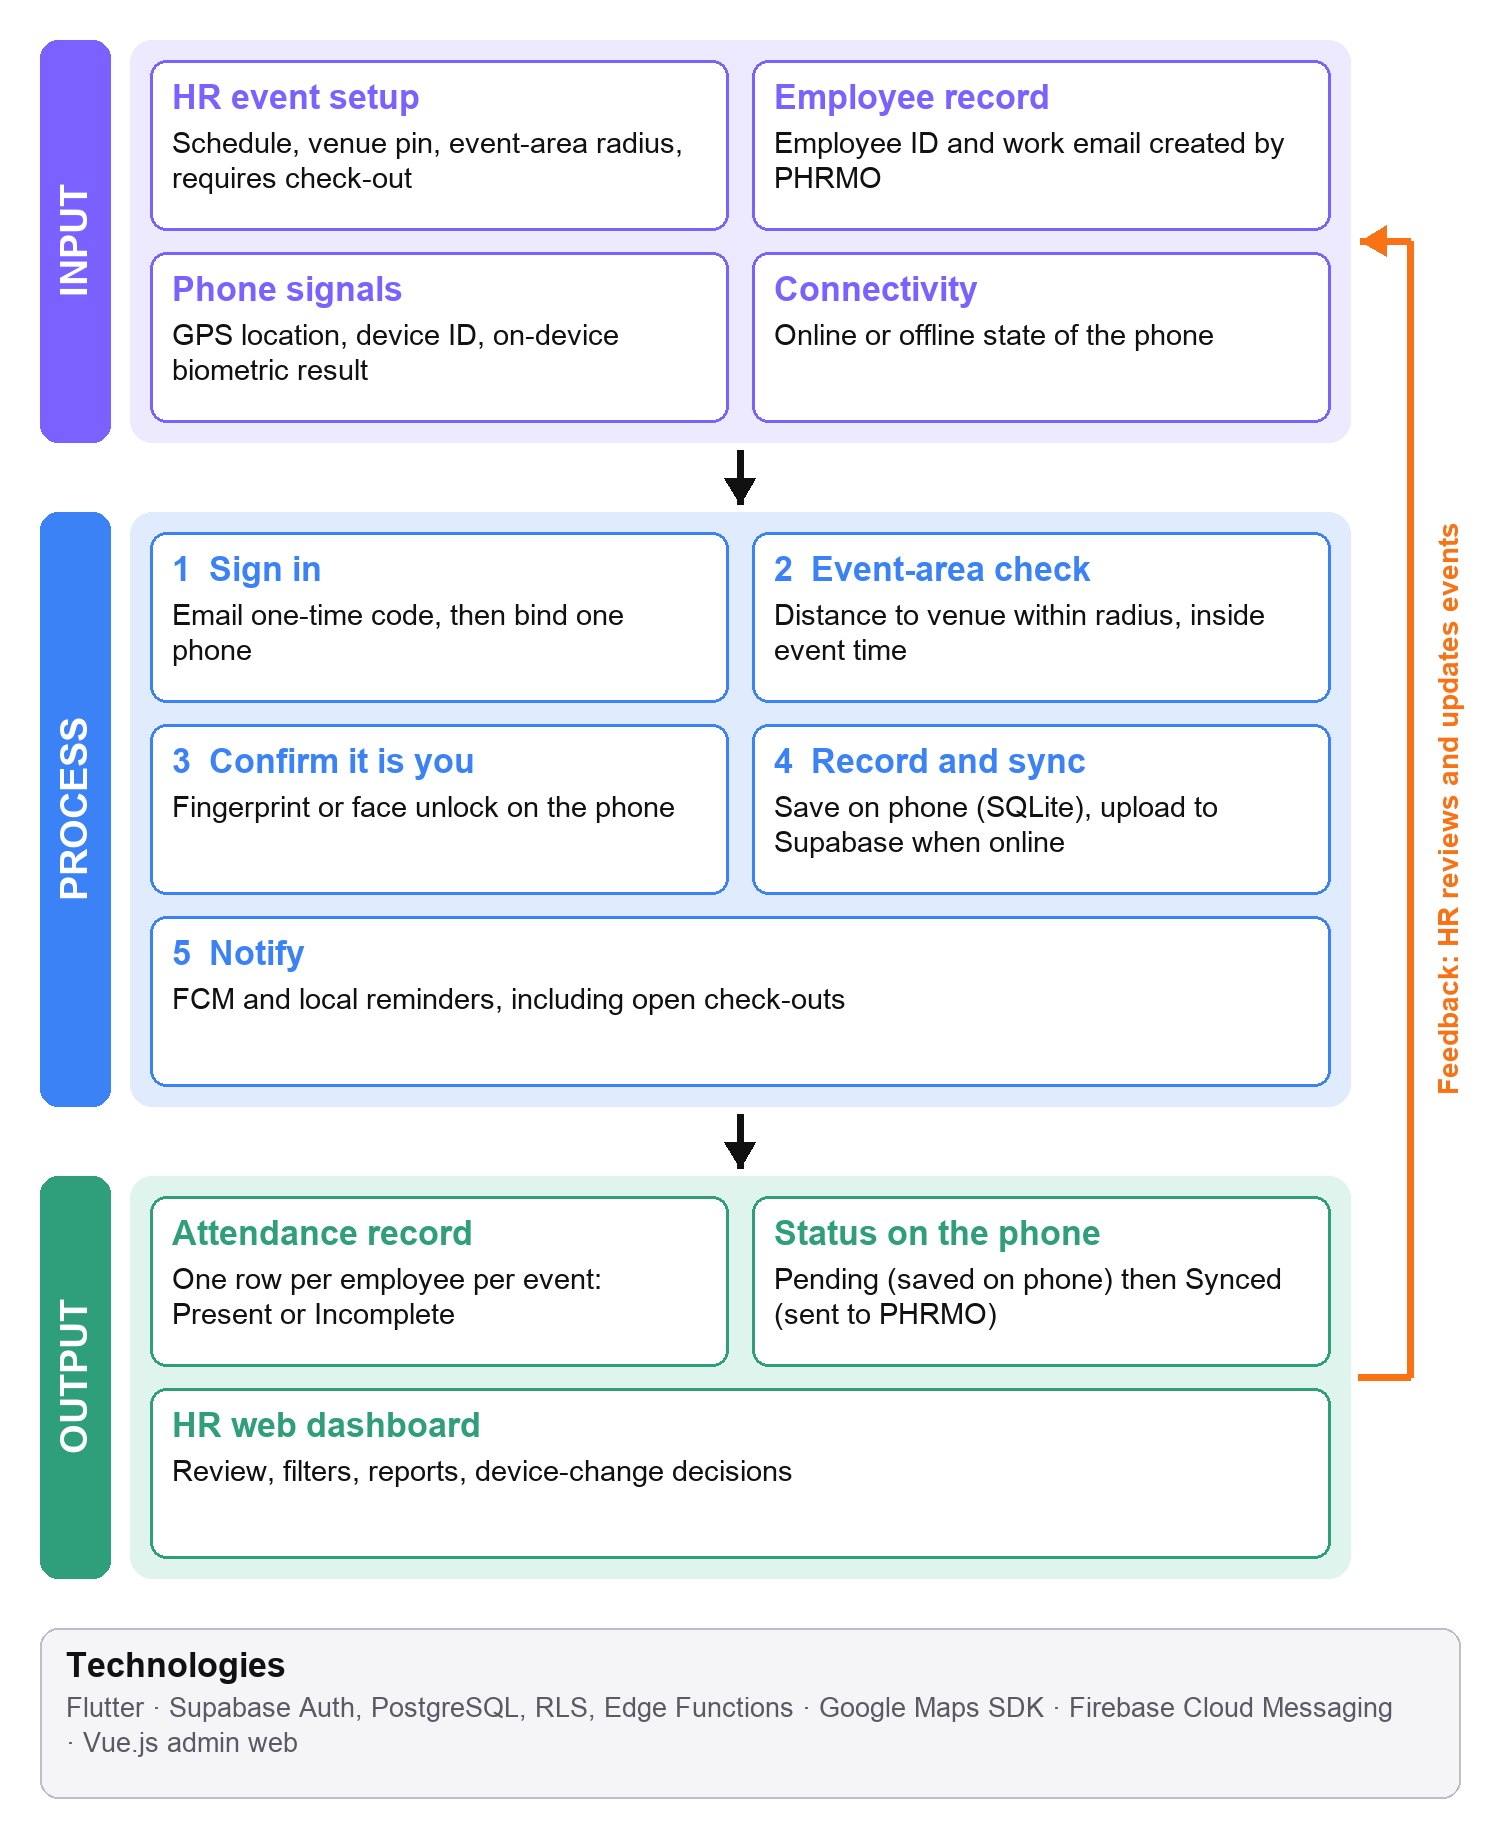
\includegraphics[
        width=\columnwidth,
        height=0.48\textheight,
        keepaspectratio
    ]{concept.png}
    \caption{Conceptual framework of PEAM-Registry.}
    \label{fig:conceptual_framework}
\end{figure}

The inputs are the event set up by HR (schedule, venue pin, event-area
radius, and whether a check-out is required), the employee record
created by PHRMO, the signals the phone provides (location, device
identifier, and the biometric result), and the phone's connectivity. The
process applies five steps in order: sign-in with an email one-time code
and phone registration; the event-area and event-time check; biometric
confirmation on the phone; recording on the phone and synchronization
to the server; and notification. The outputs are one attendance record
per employee per event, marked \textit{Present} or \textit{Incomplete};
a visible \textit{Pending} or \textit{Synced} status on the phone; and
records HR can review and report on. HR's review and event updates feed
back into the inputs. Each process step corresponds to an objective:
steps 1--3 to the first objective, step 4 to the second, step 5 and the
HR outputs to the third, and the whole loop to the evaluation in the
fourth.

\subsection{User Journey}

Figure~\ref{fig:user_journey} presents the employee user journey across
the frontend, backend, and integration layers.

\begin{figure*}[!t]
    \centering
    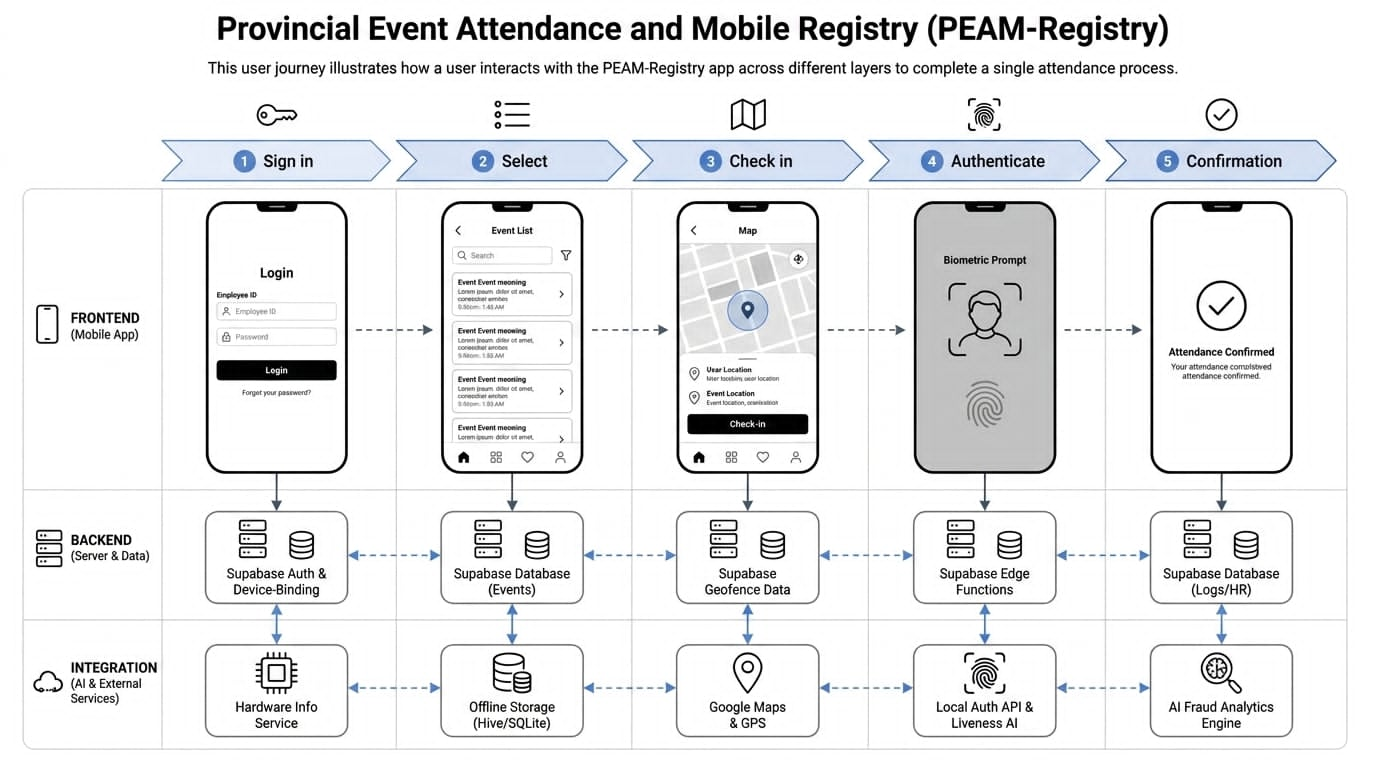
\includegraphics[
        width=\textwidth,
        height=0.42\textheight,
        keepaspectratio
    ]{userjourney.png}
    \caption{User journey of PEAM-Registry from sign-in to confirmation.}
    \label{fig:user_journey}
\end{figure*}

The primary user is a provincial employee attending an official event.
The journey begins when the employee arrives at the venue. In
\textit{Sign in}, the employee enters an Employee ID; the backend looks
up the work email PHRMO has on file, sends a six-digit code, and shows
only a masked address. A correct code starts a session and registers the
phone. Later launches on the same phone open directly. In
\textit{Select}, the employee chooses the event from a list that can be
searched and filtered by \textit{Ongoing}, \textit{Upcoming}, and
\textit{Done}; the list is cached so it opens without a connection. In
\textit{Check in}, the application reads the phone's location, shows it
on a map with the event area, and states the distance to the venue. The
button is enabled only when the event has started, has not ended, and
the employee is inside the area. In \textit{Authenticate}, the phone's
fingerprint or face unlock confirms the user. In \textit{Confirmation},
the employee sees the event, venue, time, and whether the record is
already sent to PHRMO.

Usability problems are most likely at the map (being just outside the
area), at the biometric prompt (no fingerprint enrolled), and at the
sync status (not knowing whether HR has the record). The interface
addresses these with plain sentences such as ``Move inside the event
area (within 120 m of the venue), then check your location again'' and
a short legend explaining \textit{Pending} and \textit{Synced}. The
integration layer of the figure also shows a liveness check and fraud
analytics engine; these are planned extensions and are not part of the
current build. Offline storage in the current build uses SQLite.

\subsection{System Architecture and Design}

PEAM-Registry follows a multi-client architecture in which the employee
mobile application and the HR web console share one Supabase backend
\cite{supabasedocs}. Table~\ref{tab:architecture} summarizes the
components.

\begin{table}[!t]
\caption{System Components}
\label{tab:architecture}
\centering
\footnotesize
\begin{tabularx}{\columnwidth}{@{}P{0.27\columnwidth} Y@{}}
\toprule
Component & Role and technology\\
\midrule
Employee app &
Flutter \cite{flutterdocs}; sign-in, event list, check-in and
check-out, history, notifications, profile\\
Local storage &
SQLite on the phone for attendance and a file cache for events\\
Background sync &
Android WorkManager \cite{workmanagerdocs}; uploads pending records
when the connection returns\\
Maps and location &
Device GPS through Geolocator; map display through the Maps SDK for
Android \cite{googlemapssdk}\\
Biometrics &
Platform biometric dialog through the \texttt{local\_auth} plugin
\cite{androidbiometric}\\
Backend &
Supabase Auth, PostgreSQL with Row Level Security
\cite{postgresrls}, and Edge Functions\\
Notifications &
Firebase Cloud Messaging \cite{fcmdocs} and on-device scheduled
notifications\\
HR console &
Vue.js and TypeScript \cite{vuedocs}, hosted on Vercel\\
\bottomrule
\end{tabularx}
\end{table}

The database contains departments, profiles, devices, events, event
participants, attendance records, device-change requests, and audit
logs. Three roles exist: \texttt{employee}, \texttt{hr\_administrator},
and \texttt{system\_administrator}. Each attendance record holds the
check-in and check-out times and coordinates, whether the location and
biometric checks passed, whether it was recorded offline, a
client-generated record identifier, and the time it reached the server.
A unique constraint on the event and employee pair enforces one record
per employee per event, and a database trigger sets the status to
\textit{Present} when the attendance is complete and \textit{Incomplete}
when a required check-out is missing.

Server-side logic that needs elevated access runs in five Edge
Functions so that no privileged key is shipped in the application.
\texttt{request-login-otp} and \texttt{verify-login-otp} handle the email
code and phone registration; \texttt{submit-device-change} files a
request for a new phone; \texttt{send-push} notifies employees when HR
publishes or updates an event or decides on a phone change; and
\texttt{remind-checkout} runs on a schedule and reminds employees who
checked in but have not checked out, only while the event is still in
progress.

The main data flow is as follows. HR creates an event in the web
console. The phone downloads it and caches it. At check-in the phone
creates the attendance record locally with a new client record
identifier and tries to upload it at once. If the upload fails, the
record stays \textit{Pending}, and the background worker or the next
return of connectivity uploads it. The server treats the client
identifier as unique, so a repeated upload cannot create a second
record. When the server confirms, the phone marks the record
\textit{Synced}.

\subsection{Wireframe or Interface Design}

Figure~\ref{fig:wireframe} shows the low-fidelity wireframes of the
eight employee screens. Screens 1--5 follow the user journey in
Fig.~\ref{fig:user_journey}; screens 6--8 are reached from the bottom
navigation bar and the notification bell.

\begin{figure*}[!t]
    \centering
    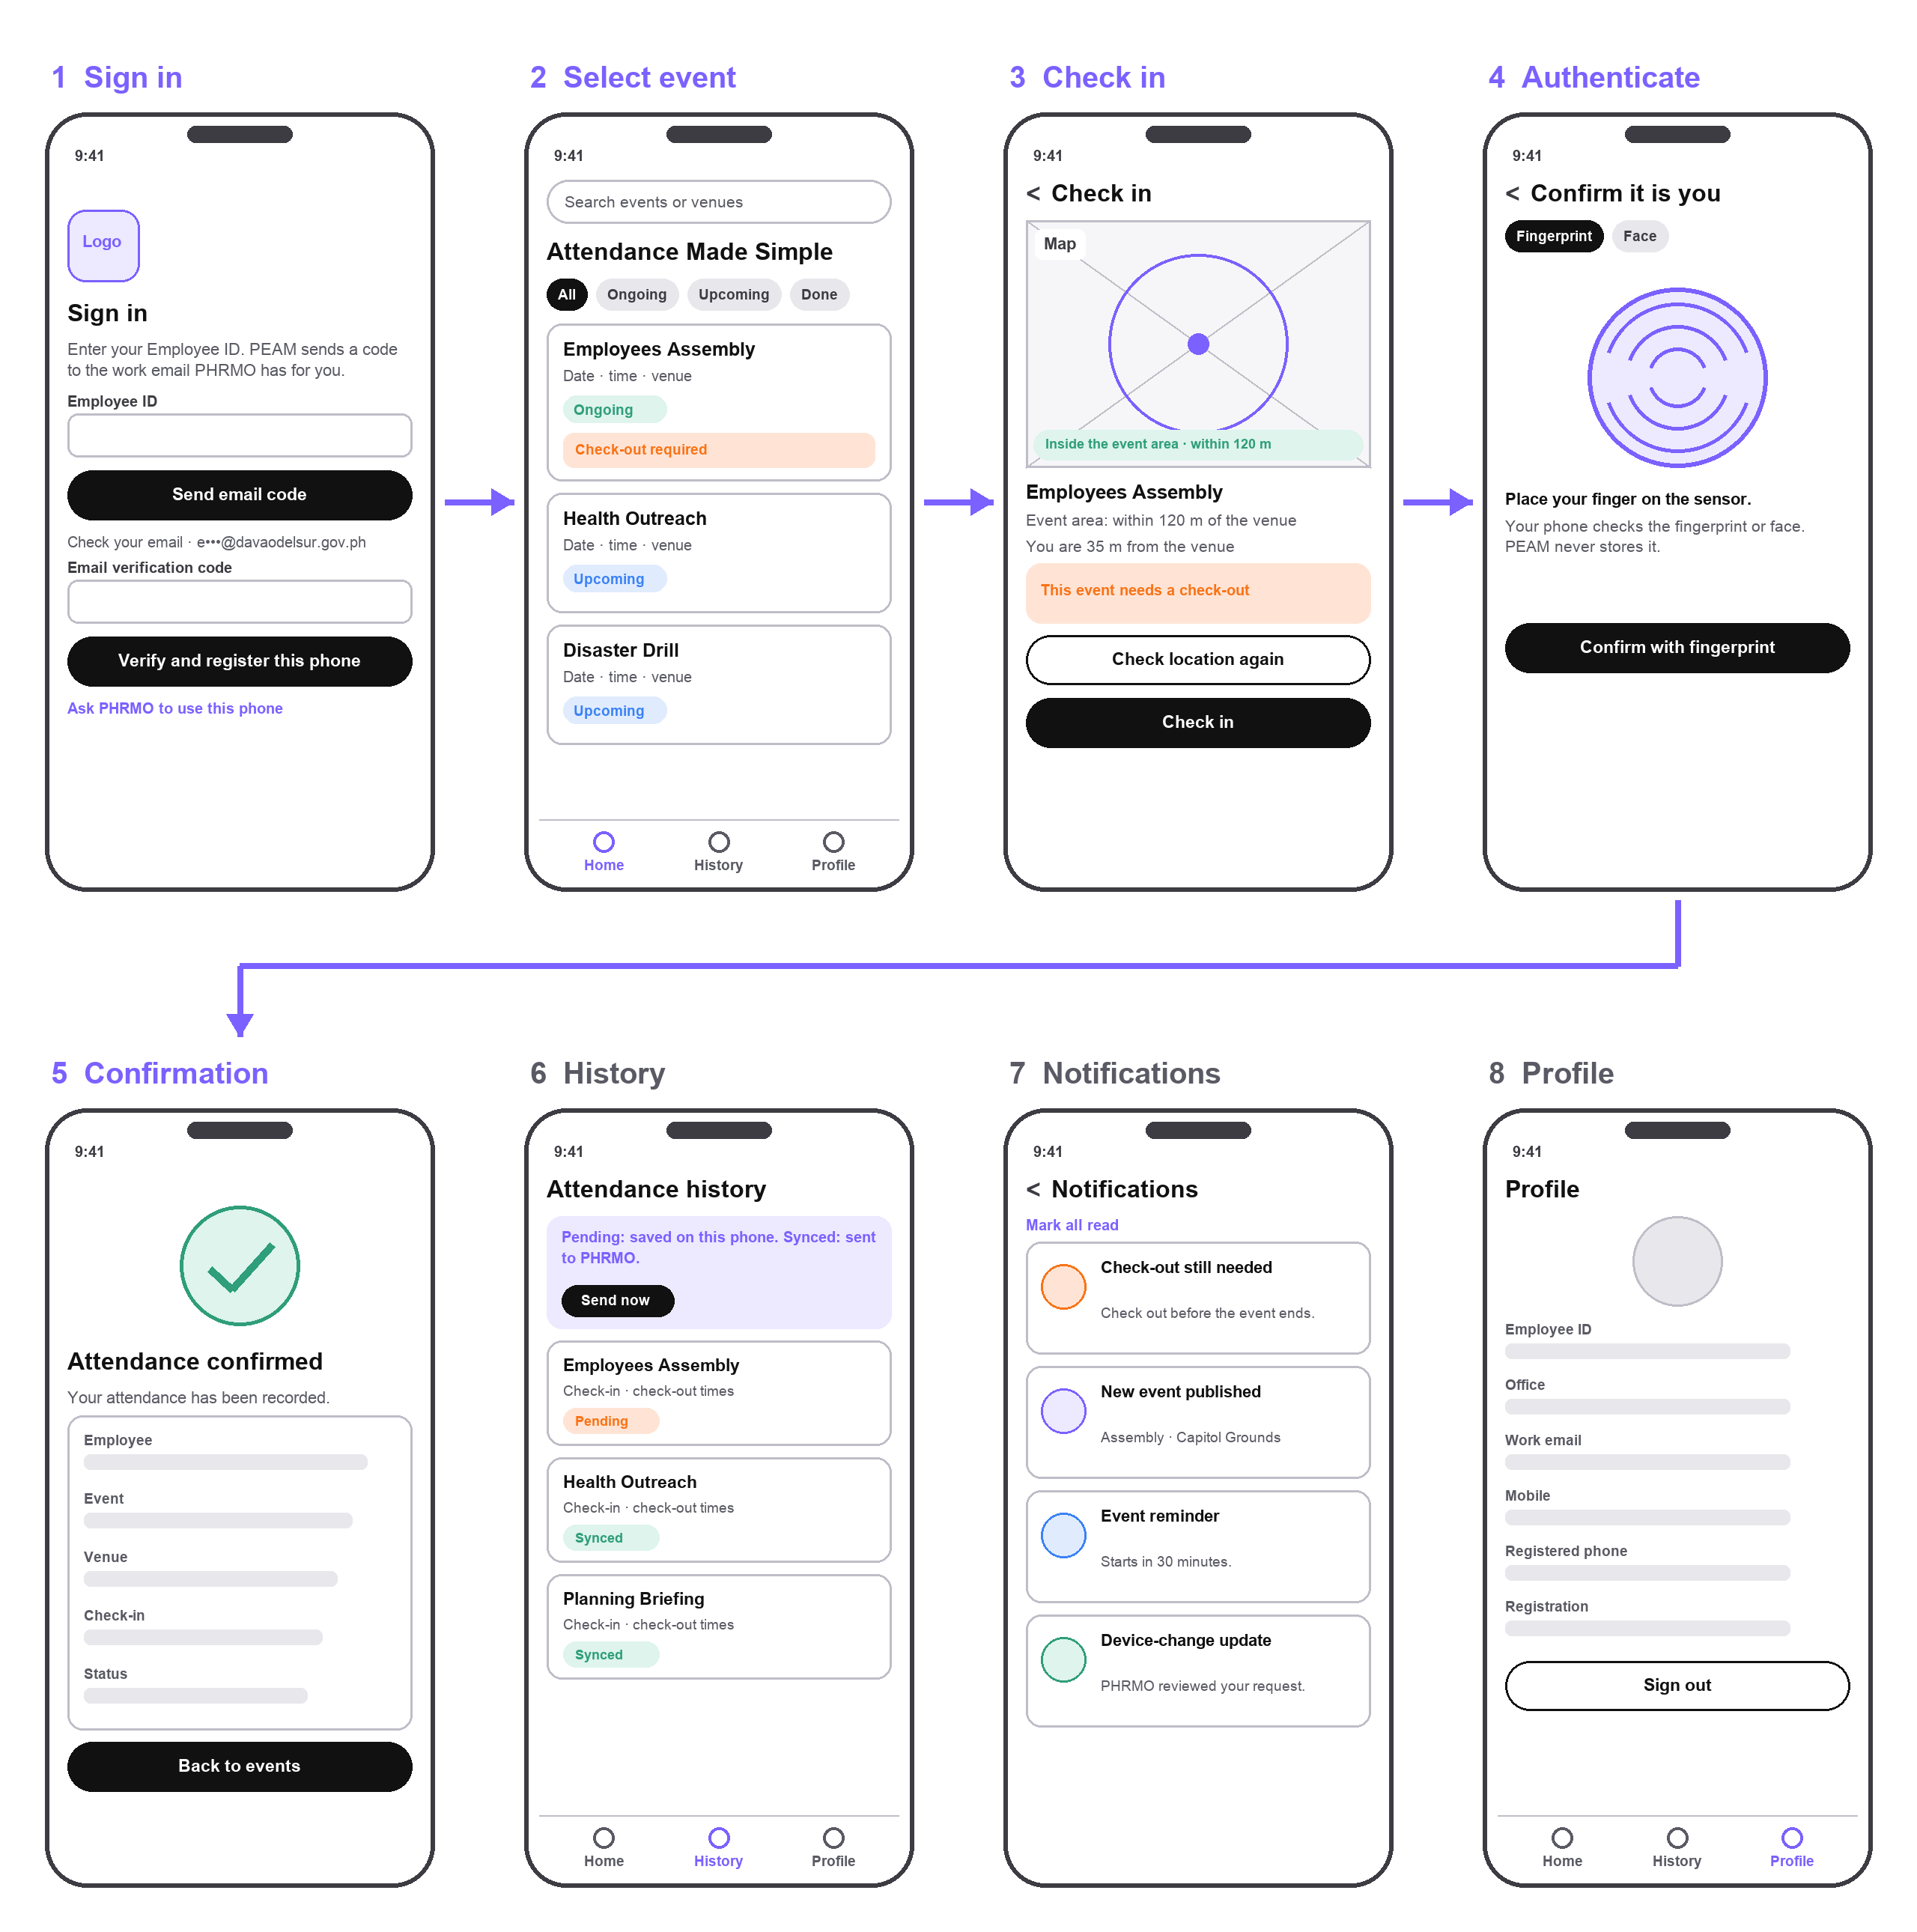
\includegraphics[
        width=0.92\textwidth,
        height=0.62\textheight,
        keepaspectratio
    ]{wireframe.png}
    \caption{Wireframes of the PEAM-Registry employee screens.}
    \label{fig:wireframe}
\end{figure*}

\textit{Sign in} asks for the Employee ID first and then the email code
on the same screen, with a link to ask PHRMO to approve a new phone.
\textit{Select event} places the search field at the top, followed by
status filters and event cards. A card for an event that needs a
check-out carries a full-width notice, ``Check-out required. Check out
before you leave.'' When a search hides events, a labeled
\textit{Clear} button and a sentence explain that other events are only
hidden. \textit{Check in} shows the map with the event-area circle, the
distance in meters, and the reason the button is disabled when it is.
\textit{Authenticate} lets the employee choose fingerprint or face only
when the phone has that method set up. \textit{Confirmation} lists the
record details and its status. \textit{History} explains
\textit{Pending} and \textit{Synced} in one sentence and offers a
\textit{Send now} button. \textit{Notifications} lists event, reminder,
check-out, and device-change notices, each of which opens the related
screen. \textit{Profile} shows the employee's office and whether this
phone is registered.

The design avoids technical terms because the users span all ages and
levels of familiarity with phones. Employee-facing text says ``event
area'' and ``within 120 m of the venue'' instead of ``geofence,'' and
``This phone is registered'' instead of ``device binding.'' Primary
actions use large, high-contrast buttons, and the brand color
(\#7B61FF) is reserved for highlights.

\subsection{Data, Participants, or Test Inputs}

\textit{Test inputs.} Development and automated tests used a fixed
sample dataset: a demonstration employee, eight provincial offices, and
four events with known dates, times, and statuses. The sample venue is
the Provincial Capitol Grounds in Digos City at
6.7492\textdegree{}\,N, 125.3571\textdegree{}\,E with a 120\,m radius.
Location tests used positions at the venue center, about 111\,m north
(inside), and far away (outside). Time tests used check-ins before the
start, during the event, and after the end. The application was run on
an arm64 Android emulator connected to the live Supabase project.

\textit{Participants.} The usability evaluation recruits five to eight
adults who are, or can stand in for, provincial employees who attend
official events \cite{virzi1992subjects}. The sample mixes office
staff who do not work in IT, three age bands (21--34, 35--49, and 50 and
above), Android and iPhone users, and people who do and do not use
phone biometrics. People who built the application are excluded.
Sessions use a demonstration account so that no real Employee ID or
inbox is exposed.

\subsection{Development and Implementation Procedure}

\begin{enumerate}
    \item \textit{Process definition.} The attendance, offline, device
    change, and notification processes were written as a step-by-step
    process document that served as the source of truth.
    \item \textit{Data design.} The PostgreSQL schema, enumerations,
    access policies, and functions such as \texttt{create\_employee},
    \texttt{bind\_employee\_device}, and the device-change approval and
    rejection functions were defined in one script.
    \item \textit{Interface design.} The user journey and wireframes
    were drafted, then implemented in Flutter with a shared component
    set.
    \item \textit{Core features.} Sign-in, phone registration, the event
    catalog with caching, the location check, the biometric step, and
    local storage were implemented in that order.
    \item \textit{Synchronization.} Upload of pending records was added
    on reconnection, on demand, and through a periodic background task.
    \item \textit{Notifications.} Firebase Cloud Messaging tokens are
    saved for the registered phone, Edge Functions send messages, and the
    phone schedules local reminders.
    \item \textit{Check-out.} Events can require a check-out, which
    repeats the location and biometric steps on the same record.
    \item \textit{Wording and accessibility review.} Employee-facing
    messages were rewritten in plain language.
\end{enumerate}

The Supabase project URL and public key are read from a local
configuration file that is not committed. Privileged keys and the
Firebase service account exist only as backend secrets used by the Edge
Functions. A continuous-integration workflow builds the Android package
on each push.

\subsection{Evaluation Procedure}

\textit{Functional verification.} The Flutter test framework was used to
write unit tests for the rules (distance, event window, reminder timing,
data mapping, sync) and widget tests that drive whole screens. The
suite runs with in-memory stores and stub location and biometric
services so that results are repeatable. The measure is the number of
tests passed out of the total.

\textit{Usability evaluation.} Each session takes about 25 minutes and
combines three methods. In a task-based evaluation following ISO
9241-11 \cite{iso9241_11}, participants perform six tasks: T1 sign in,
T2 find an event by search, T3 open check-in and read the location
result, T4 confirm with biometrics and reach confirmation, T5 find the
record in history and explain its status, and T6 open a notification.
Participants think aloud during the tasks \cite{ericsson1993protocol}.
After the tasks they complete the SUS \cite{brooke1996sus} and a short
semi-structured interview. The facilitator helps only after 60 seconds
or two failed attempts and records that task as completed with
assistance.

Effectiveness is the share of tasks completed without assistance:
\begin{equation}
E = \frac{\text{tasks completed without assistance}}{n \times k}
\times 100\%,
\label{eq:effectiveness}
\end{equation}
where $n$ is the number of participants and $k = 6$ is the number of
tasks. Efficiency is reported as the median time per task and the number
of errors and assists. Satisfaction is the mean task ease rating on a
1--5 scale and the SUS score, computed for each participant as
\begin{equation}
SUS = 2.5\left[\sum_{i\in\{1,3,5,7,9\}}(r_i - 1)
+ \sum_{i\in\{2,4,6,8,10\}}(5 - r_i)\right],
\label{eq:sus}
\end{equation}
where $r_i$ is the response (1--5) to item $i$. The result ranges from 0
to 100 and is interpreted against published benchmarks
\cite{bangor2008sus,sauro2016quantifying}. The median is reported
because the sample is small. Problems found in think-aloud and
interviews are rated on Nielsen's 0--4 severity scale
\cite{nielsen1994severity} and ranked for the next version.

\subsection{Ethical, Privacy, and Security Considerations}

The system processes personal information covered by the Data Privacy
Act of 2012 \cite{ra10173}: names, Employee IDs, work emails, phone
identifiers, and the coordinates at check-in and check-out. Collection
is limited to what attendance requires. Location is read only during a
check-in or check-out, not tracked in the background. Biometric
matching happens entirely on the phone; the application receives only
success or failure, and no fingerprint or face data is stored or sent
\cite{androidbiometric,nist80063b}.

Access is controlled at the database through Row Level Security
\cite{postgresrls}: employees can read only their own records, while HR
roles are checked through a dedicated staff function. Sign-in uses a
one-time code sent to the HR-managed email, and the application shows
that address only in masked form. Each employee may have one active
phone; a new phone requires a request approved by HR. Sensitive actions
are written to an audit log. Privileged keys never leave the server.
Usability participants give informed consent before the session, photos
are optional and separate from study consent, and participants are
identified only by codes such as P1 and P2.

% ================================================================
% III. RESULTS AND DISCUSSION
% ================================================================

\section{Results and Discussion}

\subsection{System Implementation Results}

All planned employee features and the supporting backend were
implemented. Table~\ref{tab:requirements} lists the main requirements
and their status.

\begin{table}[!t]
\caption{System Requirements and Implementation Status}
\label{tab:requirements}
\centering
\footnotesize
\begin{tabularx}{\columnwidth}{@{}l Y l@{}}
\toprule
ID & Requirement & Status\\
\midrule
R1 & Sign in with Employee ID and an email one-time code &
Done\\
R2 & One registered phone; new phone only through an HR-approved
request & Done\\
R3 & Event list with search, filters, and offline cache & Done\\
R4 & Check-in only during the event and inside the event area &
Done\\
R5 & Phone biometric confirmation; no biometric data stored & Done\\
R6 & Check-out on the same record when the event requires it &
Done\\
R7 & Offline recording with automatic sync and a visible
Pending/Synced status & Done\\
R8 & Notifications for events, reminders, open check-outs, and
device changes & Android\\
R9 & HR console for events, venue area, and attendance review &
Done\\
R10 & Role-based access enforced by the database & Done\\
\bottomrule
\end{tabularx}
\end{table}

The employee application consists of 51 Dart source files. It runs
against the live Supabase project: employees created by HR can sign in
with an email code, the phone is registered on first sign-in, events
published in the HR console appear in the list, and check-ins made
offline are kept as \textit{Pending} until they can be uploaded. The
scheduled \texttt{remind-checkout} function and the phone's local
reminder use the same timing rule, so the ``Check-out still needed''
notice is produced only while the event is running; the rule is covered
by the automated tests, and delivery on physical phones is still being
confirmed. Push notifications are limited to Android because the iOS
Firebase configuration has not been added.

\subsection{Evaluation Results}

\textit{Functional verification.} The automated suite contains 78 tests
in 11 files, and all 78 passed in the final run
(Table~\ref{tab:testsuite}). Table~\ref{tab:testcases} lists
representative scenarios drawn from those tests.

\begin{table}[!t]
\caption{Automated Test Suite Results}
\label{tab:testsuite}
\centering
\footnotesize
\begin{tabularx}{\columnwidth}{@{}Y r r@{}}
\toprule
Area tested & Tests & Passed\\
\midrule
Attendance storage, sync, check-in and check-out rules & 12 & 12\\
Background sync scheduling & 1 & 1\\
Biometric availability and messages & 11 & 11\\
Event catalog, status, and caching & 7 & 7\\
Distance and event-area check & 4 & 4\\
Sign-in and phone registration & 7 & 7\\
Notices and reminder timing & 8 & 8\\
Notification tap routing & 5 & 5\\
Server record mapping & 2 & 2\\
Configuration handling & 2 & 2\\
Screen journeys (widget tests) & 19 & 19\\
\midrule
Total & 78 & 78\\
\bottomrule
\end{tabularx}
\end{table}

\begin{table}[!t]
\caption{Representative Functional Test Cases}
\label{tab:testcases}
\centering
\footnotesize
\begin{tabularx}{\columnwidth}{@{}l Y Y l@{}}
\toprule
ID & Scenario & Expected result & Result\\
\midrule
T1 & Unknown Employee ID & Sign-in is refused with a message & Pass\\
T2 & Second phone, no approved request & Phone is not registered &
Pass\\
T3 & Registered phone relaunched & Login screen is skipped & Pass\\
T4 & Position 111\,m from center, 120\,m radius & Inside the event
area & Pass\\
T5 & Position outside the event area & Check-in stays disabled &
Pass\\
T6 & Check-in after the event ends & Check-in is refused & Pass\\
T7 & Biometric confirmation fails & Stays on the authenticate screen &
Pass\\
T8 & Check-in while offline & Saved as Pending, then Synced when online
& Pass\\
T9 & Upload fails & Record stays Pending for a retry & Pass\\
T10 & Check-out on a required event & Same record becomes Present &
Pass\\
T11 & Open check-out at 9:00 for an event ending 17:00 & Reminder set
for 16:30 & Pass\\
T12 & Open check-out after the event ends & No reminder & Pass\\
\bottomrule
\end{tabularx}
\end{table}

\textit{Usability evaluation.} The protocol, participant packet,
facilitator log, and severity worksheet are complete, and sessions with
provincial employees are being scheduled. Table~\ref{tab:usability} will
report the results; the values remain open until the sessions are
finished, so no usability scores are claimed in this paper.

\begin{table}[!t]
\caption{Usability Results (ISO 9241-11 and SUS)}
\label{tab:usability}
\centering
\footnotesize
\begin{tabularx}{\columnwidth}{@{}l Y l@{}}
\toprule
Measure & Definition & Result\\
\midrule
Effectiveness & Tasks completed without assistance,
Eq.~\eqref{eq:effectiveness} & \pending{\%}\\
Efficiency & Median time per task; errors and assists &
\pending{s}\\
Task ease & Mean rating, 1--5 & \pending{--}\\
SUS & Median (mean), Eq.~\eqref{eq:sus} & \pending{--}\\
Participants & $n$ & \pending{--}\\
\bottomrule
\end{tabularx}
\end{table}

\subsection{Analysis and Interpretation}

The functional results show that the rules that make an attendance
record trustworthy behave as designed. A check-in is accepted only when
three conditions hold at once: the event has started and not ended, the
phone is inside the event area, and the phone's biometric check passes.
Tests T4--T7 exercise each condition separately, so a failure in one
cannot be hidden by the others. The offline tests (T8 and T9) confirm the
local-first behavior described by Kleppmann et al.\
\cite{kleppmann2019localfirst}: a failed upload leaves the record on the
phone, and the client record identifier keeps a repeated upload from
creating a duplicate.

The event-area check uses the haversine distance
\cite{sinnott1984haversine} between the venue $(\varphi_1,\lambda_1)$ and
the phone $(\varphi_2,\lambda_2)$:
\begin{equation}
d = 2R\arcsin\sqrt{\sin^2\frac{\Delta\varphi}{2}
+ \cos\varphi_1\cos\varphi_2\sin^2\frac{\Delta\lambda}{2}},
\label{eq:haversine}
\end{equation}
where $\varphi$ is latitude and $\lambda$ is longitude in radians,
$\Delta\varphi = \varphi_2-\varphi_1$, $\Delta\lambda =
\lambda_2-\lambda_1$, and $R = 6\,371\,000$\,m is the mean radius of the
Earth. The phone is inside the event area when $d \le r$, where $r$ is
the radius set by HR in meters. Because smartphone positions can be off
by tens of meters indoors \cite{zandbergen2009accuracy}, HR should set
$r$ larger than the venue itself; the 120\,m default for the Capitol
grounds reflects that tolerance.

Algorithm~\ref{alg:checkin} summarizes the check-in procedure.

\begin{algorithm}[!t]
\caption{Event Check-in}
\label{alg:checkin}
\begin{algorithmic}[1]
\Require Event $e$ (start, end, center, radius $r$), employee $u$,
current time $t$
\Ensure Attendance record or a reason for refusal
\If{$t < e.\mathit{start}$ \textbf{or} $t \ge e.\mathit{end}$}
    \State \Return ``Check-in is not open for this event''
\EndIf
\State $p \gets$ current phone position
\State $d \gets$ haversine distance from $e.\mathit{center}$ to $p$
\If{$d > r$}
    \State \Return ``Move inside the event area, then try again''
\EndIf
\If{phone biometric check fails}
    \State \Return ``Could not confirm it is you''
\EndIf
\State $a \gets$ new record for $(u, e)$ with time $t$, position $p$,
and a new client record ID
\State Save $a$ on the phone as \textit{Pending}
\If{the phone is online \textbf{and} upload of $a$ succeeds}
    \State Mark $a$ as \textit{Synced}
\EndIf
\State \Return $a$
\end{algorithmic}
\end{algorithm}

The check-out reminder applies the same concern for timing. A reminder
after the event is useless, so the system schedules it only between the
start and the end. Algorithm~\ref{alg:reminder} gives the rule used by
both the phone and the server function.

\begin{algorithm}[!t]
\caption{Check-out Reminder Timing}
\label{alg:reminder}
\begin{algorithmic}[1]
\Require Event start $s$, end $f$, check-in time, current time $t$
\Ensure Reminder time, ``now,'' or none
\If{check-out not required \textbf{or} already checked out
\textbf{or} $t < s$ \textbf{or} $t \ge f$}
    \State \Return none
\EndIf
\State $q \gets f - 30$ minutes
\If{$q \le s$} \Comment{short event}
    \State $q \gets s + (f - s)/2$
\EndIf
\If{$q > t$}
    \State \Return $q$
\ElsIf{$f - t < 2$ minutes}
    \State \Return none
\Else
    \State \Return now
\EndIf
\end{algorithmic}
\end{algorithm}

Several limitations remain. The application trusts the position the
operating system reports and does not yet detect mock-location tools.
The biometric step confirms that someone enrolled on the phone unlocked
it; it cannot tell apart two people who both enrolled on the same phone,
which is why the one-phone rule and HR review matter. Testing was
carried out on an emulator with simulated positions, so accuracy at real
venues still needs field confirmation. Finally, satisfaction and
efficiency cannot be judged until the usability sessions are complete.

Table~\ref{tab:comparison} compares PEAM-Registry with the two methods
it is meant to replace for off-site events.

\begin{table*}[!t]
\caption{Comparison of Off-Site Attendance Methods}
\label{tab:comparison}
\centering
\footnotesize
\begin{tabularx}{0.96\textwidth}{@{}lYYYYY@{}}
\toprule
Method & Setup at the venue & Identity & Presence at venue & Without
internet & Main limitation\\
\midrule
Paper sign-in sheet & Print and bring sheets & Signature only & Not
shown & Works & Easy to sign for others; manual encoding\\
Transported biometric scanner & Carry, power, and configure a device &
Fingerprint on scanner & Implied by the device location & Works; logs
downloaded later & Equipment, queues, delayed records\\
PEAM-Registry & None; HR sets the event area in advance & Phone
biometric on a registered phone & Distance to venue checked each time &
Saved on phone, synced later & Depends on GPS accuracy; mock locations
not yet detected\\
\bottomrule
\end{tabularx}
\end{table*}

\subsection{Discussion of Research Objectives}

\textit{Objective 1} was achieved. Check-in requires the event window,
the event area, and the phone's biometric confirmation, and the system
allows only one registered phone per employee, as shown by
requirements R2, R4, and R5 and tests T2 and T4--T7.

\textit{Objective 2} was achieved. Attendance is saved on the phone,
uploaded automatically when the connection returns, and limited to one
record per employee per event, as shown by R6 and R7 and tests T8--T10.

\textit{Objective 3} was achieved for Android. The shared backend and
HR console are in place, and notifications are implemented for
published events, event reminders, open check-outs, and device-change
decisions, with the reminder timing verified by T11 and T12. Delivery
on physical phones and iOS notifications remain outstanding.

\textit{Objective 4} was partially achieved. Functional verification is
complete, with 78 of 78 tests passing. The usability evaluation is
designed and ready, but its results are not yet available.

% ================================================================
% IV. CONCLUSION
% ================================================================

\section{Conclusion}

This study addressed the lack of a portable and trustworthy way to
record attendance at provincial events held away from the Capitol. It
produced PEAM-Registry, a Flutter application with a Supabase backend and
an HR console, in which an employee's own registered phone confirms both
presence and identity. A check-in is accepted only during the event,
only inside the event area, and only after the phone's biometric
check, and it is saved on the phone first so that a poor connection
does not lose it. Notifications, including a check-out reminder that is
sent only while the event is still running, help employees finish their
attendance. All 78 automated tests passed, which shows that these rules
behave as specified. The main contribution is a single workflow that
combines the event window, the event area, on-device biometrics,
one phone per employee, and offline-first synchronization for a local
government setting, without collecting biometric data.

\subsection{Recommendations and Future Work}

\begin{enumerate}
    \item Complete the usability sessions with five to eight provincial
    employees, report effectiveness, efficiency, and SUS, and fix
    high-severity problems before a field trial.
    \item Run a pilot at a real off-site event and compare the time to
    record attendance and the number of disputed records with a
    transported scanner.
    \item Detect mock-location tools and record the reported position
    accuracy, so that low-accuracy check-ins can be flagged for HR.
    \item Configure Firebase for iOS and test the full journey on
    iPhones.
    \item Add the planned liveness check and fraud analytics only if
    they can run without storing biometric data, and evaluate their
    effect on false rejections.
    \item Sign release builds with a dedicated release key before wider
    distribution.
\end{enumerate}

% ================================================================
% REFERENCES
% ================================================================

\printbibliography

\end{document}
